\begin{frame}[fragile]{GNU Radio Installation (6/7)}

\footnotesize

\begin{itemize}
    \item \textbf{Verify the VOLK Installation.}

    \begin{itemize}
        \item VOLK (Vector-Optimized Library of Kernels) is a GNU Radio library that
        optimizes signal processing operations by selecting the fastest SIMD
        implementation (e.g., AVX, AVX2, AVX-512, NEON) for the host processor.
    \end{itemize}
\end{itemize}

\scriptsize

\begin{center}
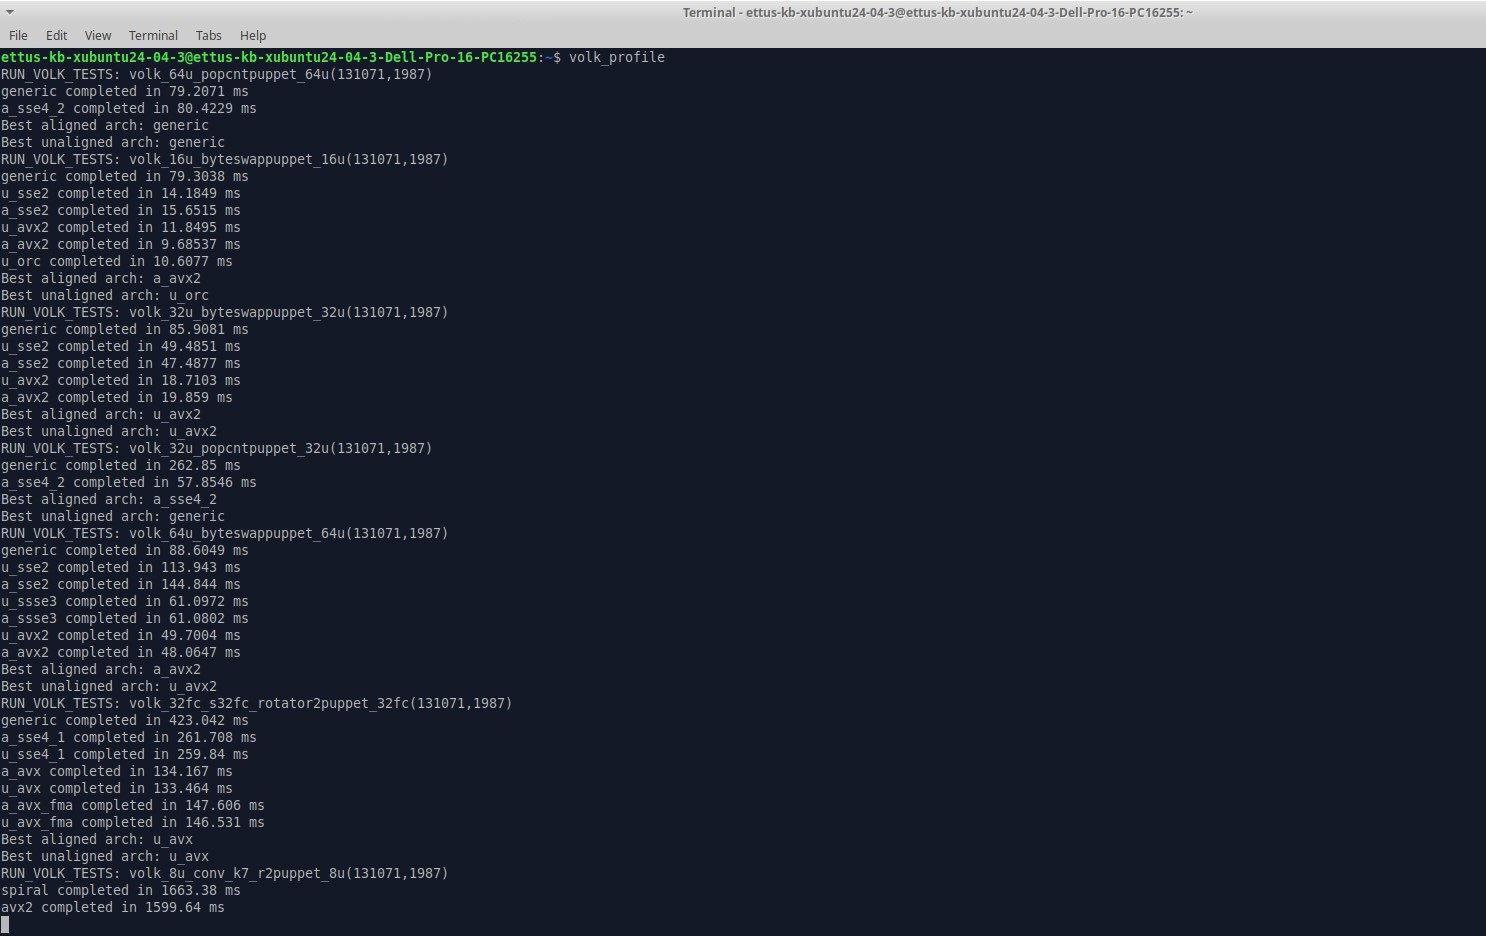
\includegraphics[
    width=0.8\linewidth,
    height=0.62\textheight,
    keepaspectratio
]{latex/jpg_png/image_Volk profile output.jpg}
\end{center}

\end{frame}